\section{Introduction}
% 1. Describe the Current Situtation
% Functions as a starting point and a common basis. Therefore it primarily contains recognizable and agreed points.
% 2. What is the complication, challenge identified
% Spells the reason for acting now. It contains threats / opportunities and the hurdles that need to be overcome.
Technological advances in hardware that augment a user's physical actions have reignited dreams of overcoming human limitations, recovering lost abilities as well as simplifying skill acquisition. Wearable exoskeletons move a user's body by applying forces to the extremities, for example by pulling on the fingertips (see Dexmo Haptic Glove \footnote{https://www.dextarobotics.com/}) while electrical muscle stimulation (EMS) makes the user's extremities move by sending current into the muscle activating nerves. These technologies are becoming increasingly seamless to use. However, augmented user's frequently report dissociative experiences following augmented action. They do not experience agency.

The sense of agency refers to the experience of being in control of our own voluntary actions, instead of them feeling as though they randomly happen to us. This being in the "driving seat when it comes to our own actions"~\cite{Moore2016-ub} can be subdivided into the \textit{feeling} of agency, a low level pre-reflective sensory process, and a more higher level reflective cognitive process, the \textit{judgement} of agency~\cite{Moore2016-ub, Danry2022-xk}. The key challenge in human \textit{physical augmentation} is to create an experience of pre-reflective agency, so user's feel as though they are in the "driving seat" once again.
% if something happens for you in an interaction there is a cost to that:
% - impacts sense of agency which in turn makes user's engage less
% - impacts precision and accuracy, which can be very critical in high stakes scenarios, e.g. air traffic control

% 3. Question
% Asks the question how the hurdles of the Complication can be overcome. How can we prevent the threat or seize the opportunity? Also, what would be the benefits if the complication would be overcome?
% What have others done to address this and what do we propose "instead"
In physical augmentation, this experience of agency positively impacts performance.~\citet{Kasahara2019-sk} have shown that reaction times when tapping targets on a touchscreen can be increased by augmenting the user. Critically they found an optimal increase in reaction time, \textit{pre-emptive} gain, that preserves agency. At around 80 ms preceding the naturally occurring action, user's integrate the augmentation and maintain an experience of agency. However, setting this gain factor is dependent on each specific task and requires fitting the parameters over and over again. A key question remains: How can we maintain agency during physical augmentation without training and over-fitting parameters? In other words, how can we create closed systems for users to experience natural augmentation?

% 4. (short) Answer Teaser
% Provides the answer on how to overcome the hurdles. Explains how this will help deflect the threats or seize the opportunities.
% keep this short
In this paper, we present a system that establishes a fast communication channel between the user's brain signals and a physical end effector, here EMS. The system controls the user's muscles through EMS at the time of the user's intent to interact, as measured through readiness potentials (RP) present in the user's electroencephalogram (EEG). In our user study we then applied a mixed-methods research approach to investigate whether keeping the physical impact on the user's body in line with their intention to move, preserves their sense of agency.

\subsection{Preserving Agency using Brain Signals of the Intent to (Inter)act}
% 4. (long) Anwser with teaser image
% Provides the answer on how to overcome the hurdles. Explains how this will help deflect the threats or seize the opportunities.

%- not only physical integration but also other adpative interfaces, or control of mobile phone
\missingfigure{maybe small infographic here showing the connection from EEG volitional RP thought to EMS trigger on the Arm. <- better use this for the teaser image. Here better present the main results, i.e. sense of agency scores?}

% This is what most people (90+%) will see from your paper!

% - [ ]  use hemingwayapp.com (+SEO if hardcore) to make figure captions super precise
% - [ ]  are all the axes labels readable, font size 10 or up
% - [ ]  check for missing information: give someone the figure with captions to someone neutral to check if everything is clear from the figure alone
% - [ ]  for digital version: what is alt-text of figure, i.e. when hovering with the mouse over the figure what text appears next to the cursor
% - [ ]  for accessibility: write figure caption for the blind
%     - [ ]  explain what the figure shows
%     - [ ]  refactor using hemingwayapp.com

\begin{teaserfigure}
  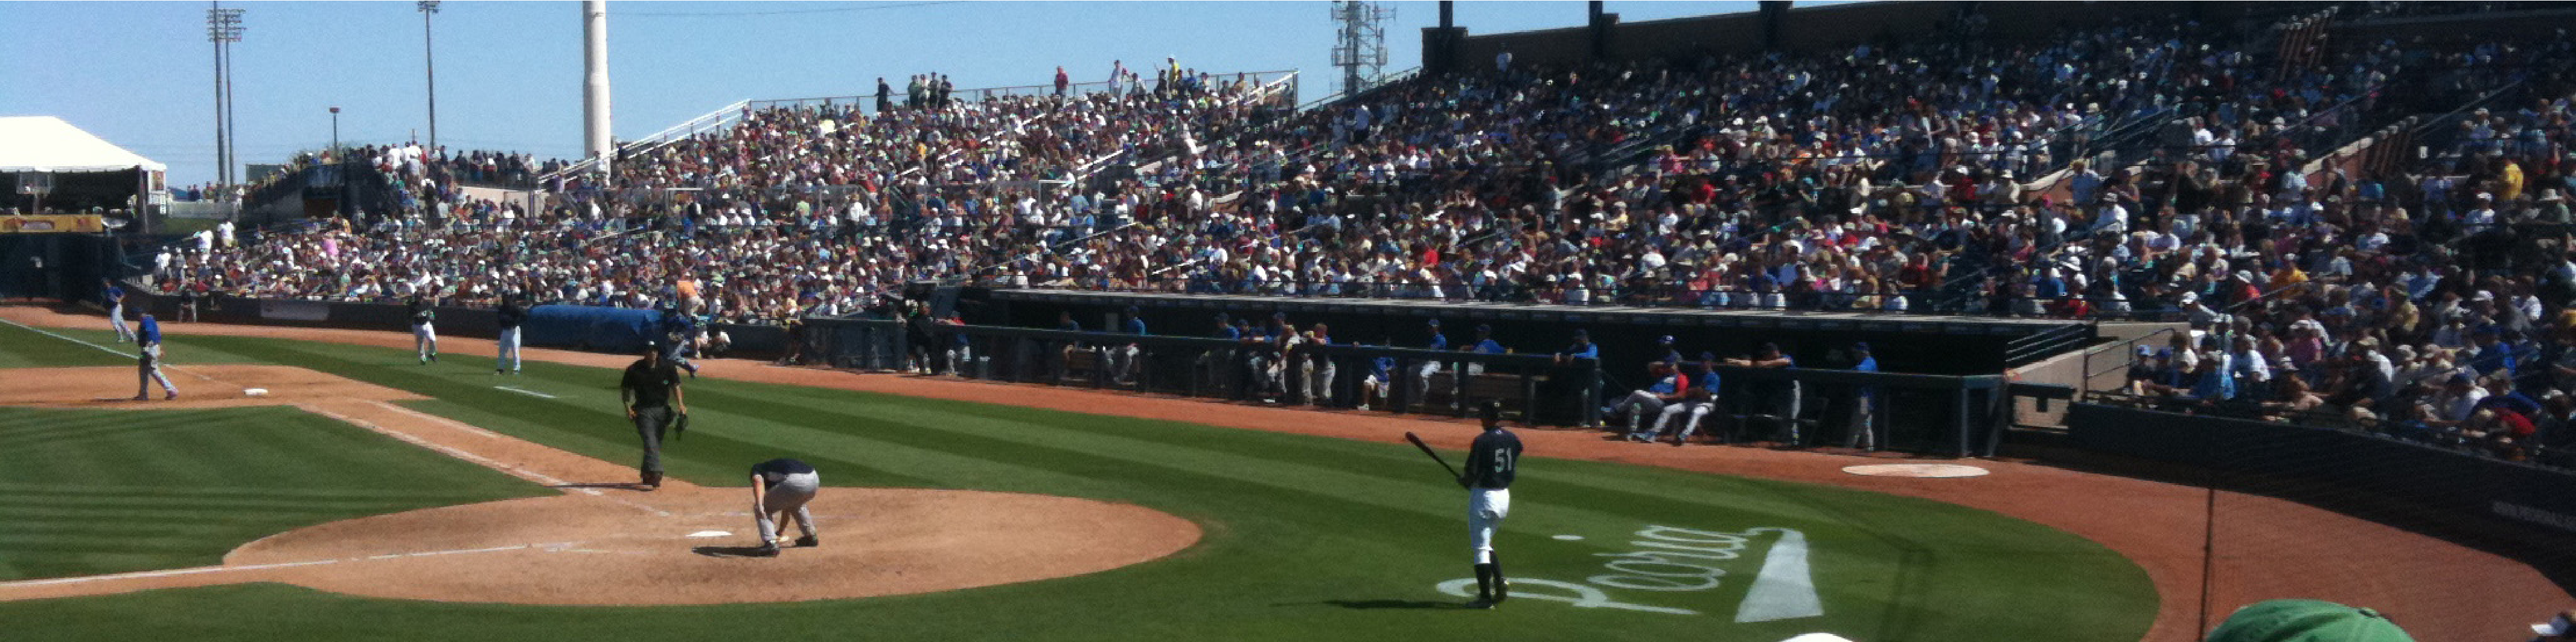
\includegraphics[width=\textwidth]{tex_sample_files/sampleteaser.pdf}
  \caption{Seattle Mariners at Spring Training, 2010.}
  \Description{Enjoying the baseball game from the third-base
  seats. Ichiro Suzuki preparing to bat.}
  \label{fig:teaser}
\end{teaserfigure}